\documentclass[10pt,letterpaper]{article}
\usepackage[notes,backend=biber]{biblatex-chicago}

%% Language and font encodings
\usepackage[english]{babel}
\usepackage[utf8x]{inputenc}
\usepackage[T1]{fontenc}

%% Sets page size and margins
\usepackage[a4paper,top=3.5cm,bottom=2cm,left=3.5cm,right=3cm,marginparwidth=1.75cm]{geometry}

%% Other Packages
\usepackage{rotating}

%% Useful packages
\usepackage{amsmath}
\usepackage{graphicx}
\usepackage[colorinlistoftodos]{todonotes}
\usepackage[colorlinks=true, allcolors=blue]{hyperref}
\bibliography{bibliography.bib}



%% Title
\title{
		\usefont{OT1}{bch}{b}{n}
		\normalfont \normalsize \textsc{APC 524: Final Project Report} \\ [10pt]
		\huge 2D Motion Planning \\
}
\selectlanguage{english}
\usepackage{authblk}
\author[1]{Kevin Andrade}
\author[2]{Benjamin Laitner}
\author[3]{Lap Hei Lam}
\author[4]{Salman Sarwar}
\author[5]{Michelle Zhang}
\affil[]{Princeton University}


\begin{document}
\maketitle

\begin{abstract}
\noindent This project is centered around the path-planning problem which arises in various fields across robotics, biology, and autonomy. The algorithms implemented for the path planning aspect of the program include Rapidly-Exploring Random Trees and A*. This was done in environments with circular, rectangular, and circular obstacles, and were navigated using an Unmanned Aerial Vehicle (UAV) represented by a circle. 
\end{abstract} \\ 

\tableofcontents
\newpage


\section{Introduction}

In recent decades, there has been a tremendous proliferation of autonomous vehicles such as self-driving cars and self-navigating drones and robots. Although there are many branches of science at work that enable these complex systems to continuously improve, one important component is the path-planning algorithm. Path-planning algorithms are critical when it comes to deploying autonomous vehicles because they enable the vehicles to be able to go from one point to another while navigating around obstacles. Such autonomous vehicles are able to leverage path-planning algorithms by collecting information through cameras and use the gathered information in clever ways. 
Generally, it is desired for the robot to reach a specific goal from wherever its origin point may be within a 2D or 3D space. In a realistic setting, there are often obstacles these vehicles must be able to circumvent while on their way to the destination. The existence of such obstacles makes it difficult for vehicles to go from their origin to their desired destination, thus requiring careful selection of an algorithm. Ideally, the algorithm is able to carve out a path for the vehicle to follow, spanning from its current location to its desired destination.
In real systems, resources come at a premium. Within this project, we hope to be able to build a software package that enables users to explore the trade-offs of utilizing different path-planning algorithms with different vehicles in both static and dynamic environments. For now, we will utilize A* and RRTs given that each of these algorithms have their own pros and cons.

\section{Project Goals}
We aim to construct a modular, robust software package implementing trajectory motion planning for an arbitrary vehicle in a possibly dynamic, user-defined environment; given an arbitrary dynamical environment along with a dynamical agent, we search for a feasible and/or possibly optimal path between an initial state and a goal state. 



\begin{sidewaysfigure}
    \centering
    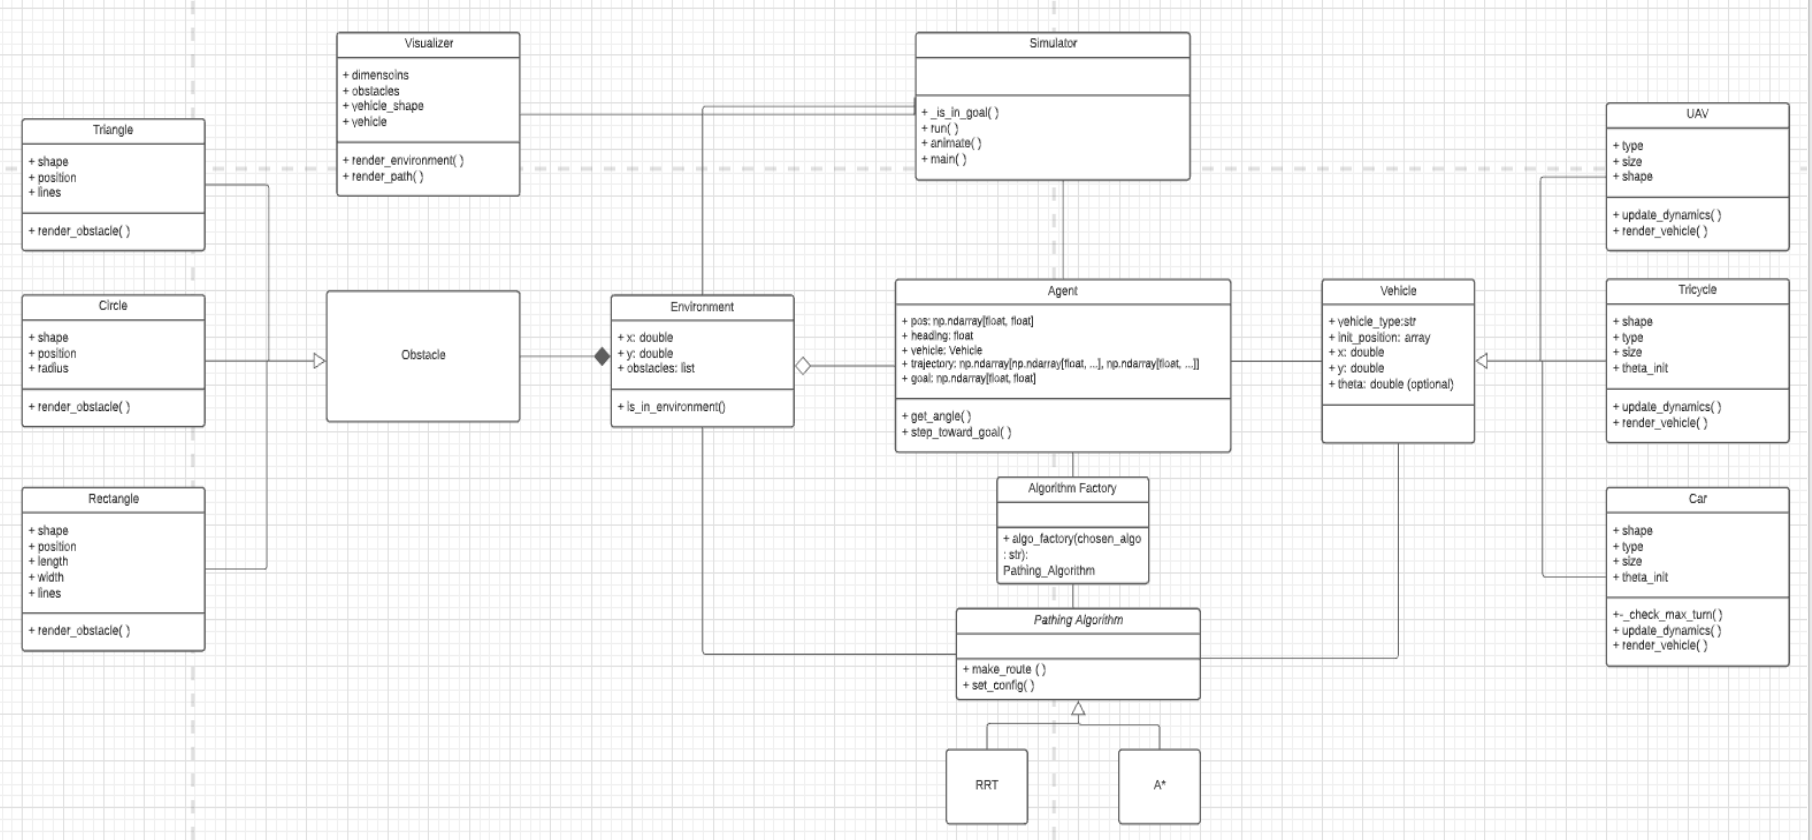
\includegraphics[width= 27 cm]{figures/UML.png}
    \caption{UML Diagram}
    \label{fig: UML}
\end{sidewaysfigure}


\subsection*{Overview of Our System's Functionality}
The system will include the following options:
\begin{itemize}
    \item Type of Path-Finding Algorithm
    \item Type of Obstacles
    \item Dynamic and Static Obstacles 
    \item Type of Vehicle
\end{itemize}

\section{Theoretical Background - Motion Planning}

At a high level, the general motion planning problem can be stated as follows: given two states $x_1$ and $x_2$, does a path exist from $ x_1 \rightarrow x_2$ that respects obstacles and the dynamics of the vehicle? If so, can we find an optimal path under some performance metric? We focus our attention on two algorithms: Rapidly-Exploring Random Trees (RRT), concerned with feasible paths, and A$^*$, concerned with optimal paths.


\subsection{Rapidly-Exploring Random Tree (RRT)}

\begin{figure*}[!h]
    \centering
    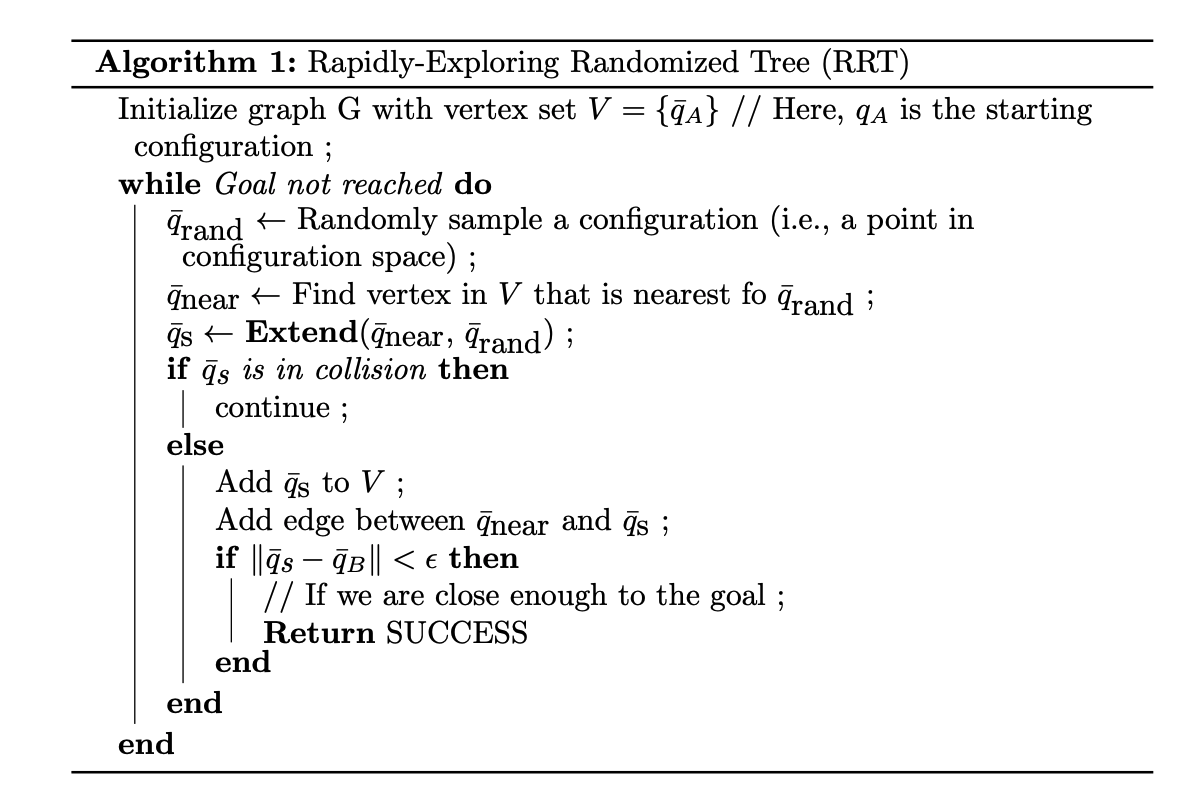
\includegraphics[width= 11 cm]{figures/rrt.png}
    \caption{RRT Algorithm }
    \label{fig: rrt}
\end{figure*}

\noindent RRT is an algorithm that is guaranteed to find a solution, albeit not optimally. The algorithm is run iteratively for a pre-specified. number of times, where then a path is constructed to the desired goal if one exists, barring extreme conditions (such as the goal being completely surrounded by obstacles). For every iteration, a random point is sampled within the environment; if the sampled point is in collision with one of the obstacles, then the point is sampled until a sampled point that is not in collision with an obstacle is found. Once this sampled point is established, then a list of vertex is checked to find a previously visited point that is the closest to the sampled point. The distance between this vertex and the sampled point is calculated, where if the distance is less than the specified step size, then a new connection is established where the vertex becomes the parent point of the sampled point and the sampled point gets added to the list of vertices so that it can be used in the future to get close to other sampled points in the future. However, since in this case we are dealing with robots that have an actual shape, collision at the sampled point must be checked. If there is no collision between the vehicle and obstacles at the sampled point, then the sampled point can be added to the list of vertices. However, if there is a collision, then the sampled point does not get added to the list of vertices and the algorithm moves on to the next sampled point, where it then repeats the process.\\

\noindent To check if there are collisions between the vehicle and obstacle, a variety of different functions are deployed; a variety of functions are required because of the different shapes that represent the vehicles and obstacles. If the vehicle is represented as a circle, then collisions are easy to detect when it comes to circle obstacles. The way to calculate this is by calculating the sum and differences of the radii of the two circle and then seeing if the distance between the two centers of the circle are in between these two quantities. If the distance is indeed between these two quantities, then that means the circles intersect and that there is a collision between the vehicle and obstacle. This function is represented by the function circle\_\circle\_\collision(). To check if the circular vehicle does not collide with the polygon obstacles (i.e. the rectangle and triangle obstacles), three different conditions must be satisfied. The first condition that must be met is that there are no intersections between the circle and any of the lines associated with the polygon. This is done with the function line\_\circle\_\intersect(), where it checks if the nabla is zero or not. The second condition that must be satisfied is to see if the center of the circular vehicle is inside the polygon obstacle. This covers the corner case where the vehicle is initialized inside a large polygon. This is done with the function is\_\inside\_\circle. The third condition that must be satisfied is to see if the circle does not intersect with any of the lines associated with the polygon and the center of the circle is not in the polygon, then the distances between the vertices of the polygon and the center of the circle must be checked so that it is not shorter than the radius of the circle. This checks the situation when the initialized vehicle is so big that it does not intersect the sides of the polygon and its center is able to not be inside the polygon. If all three of these conditions are satisfied, then the vehicle is not in collision with the obstacle. However, if at least one of the conditions is violated, then the vehicle is in collision with an obstacle.\\ 

\begin{figure*}[!h]
    \centering
    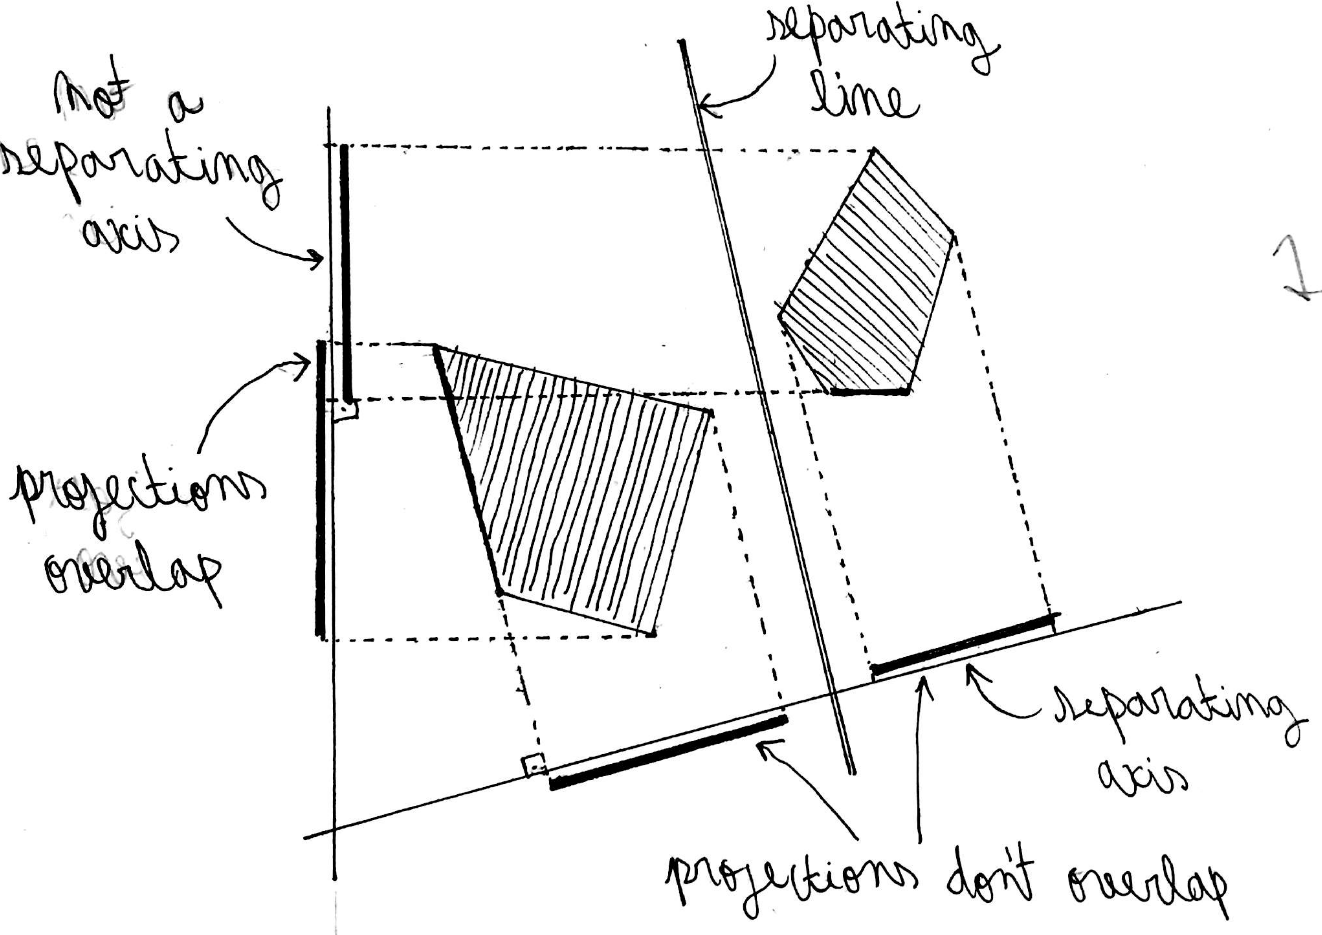
\includegraphics[width= 11 cm]{figures/SAT.png}
    \caption{Depiction of SAT}
    \label{fig: sat}
\end{figure*}

\noindent In the case where the vehicle is a rectangle, collisions between the vehicle and a circular obstacle can be found by utilizing the same function that was used to check the three different conditions between the circular vehicle and polygon obstacle in the case above. For collisions with polygon obstacles, different functions were used. To test collisions between a rectangular vehicle and a rectangle or triangle obstacle (and more generally collisions between convex polygons), the separating axis theorem (SAT) is used. The idea behind the theorem is to find if there exists a line that can run between the two polygons without intersecting either of them. This is done by taking the normal vectors of each edge of each polygon and projecting them onto a line. If all the pairs of projections of the all the edges overlap, then the two polygons. Otherwise, there is no intersection between the two polygons.

\begin{figure*}[!h]
    \centering
    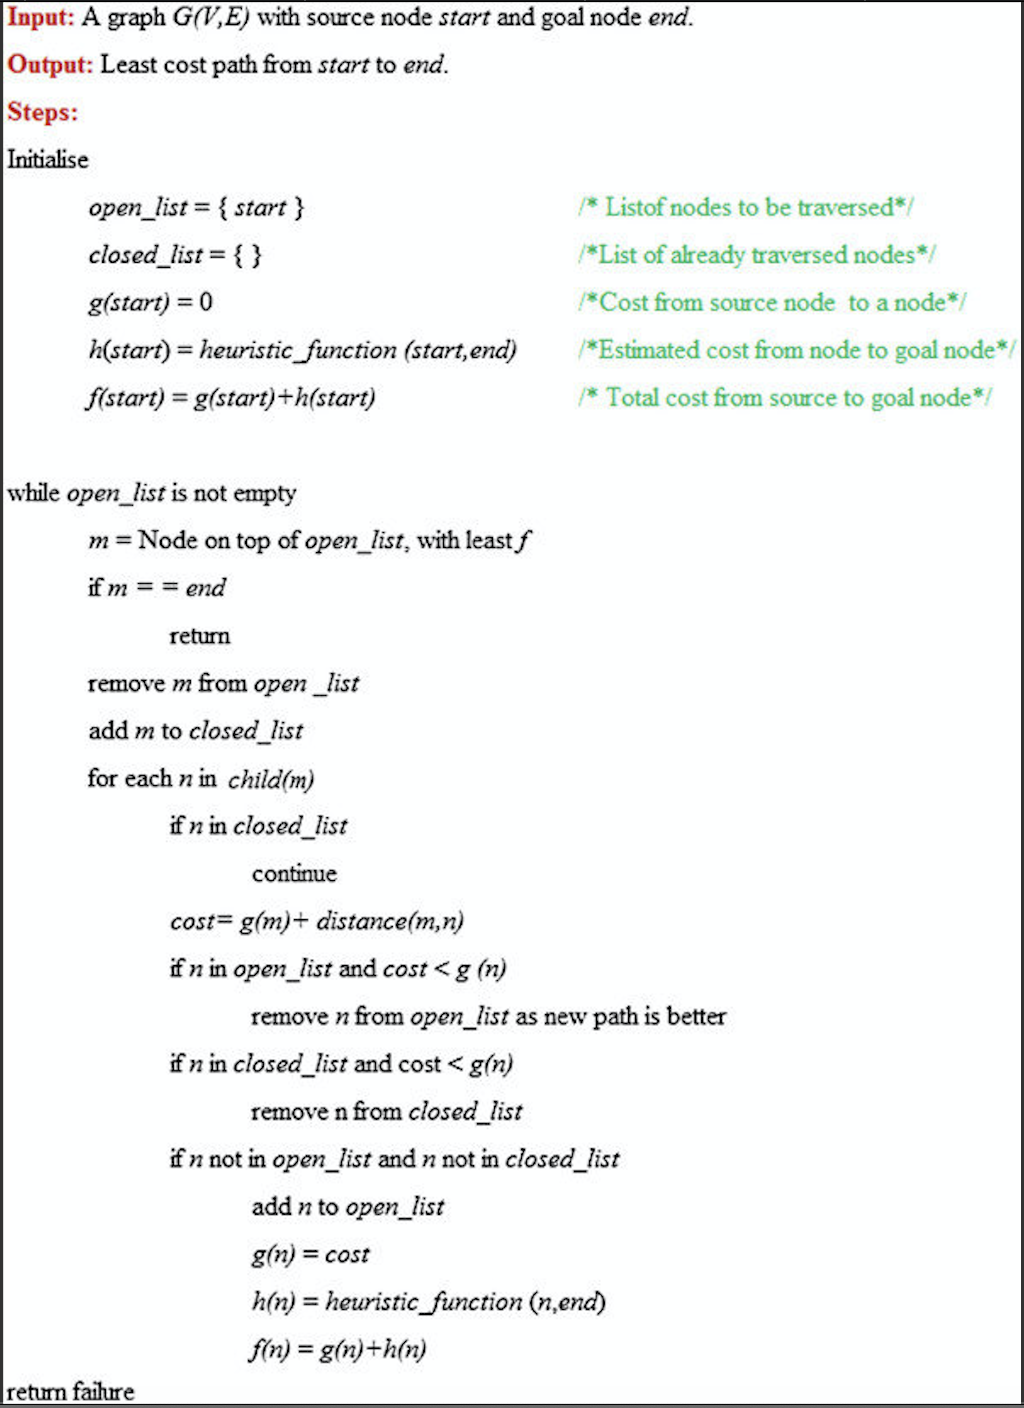
\includegraphics[width= 7.5 cm]{figures/astar.png}
    \caption{Pseudocode structure of the A* algorithm.}
    \label{fig: a_star}
\end{figure*}


\subsection{$A^*$ Algorithm}

    \subsubsection*{Formulating the problem}
    
    Motion planning in discrete spaces can be formulated in the language of state space models. The fundamental idea is that each unique robot configuration is called a state, and the set of all possible configurations is the state space $X$. We can act on a state with an action $u$ to produce new states $x' = f(x,u)$, where $f$ is termed a \textit{state transition function}. We define initial and goal states $x_I, x_G \in X$; the planning problem then reduces to finding a series of actions to transform $x_I \rightarrow x_G$. 
    
    In our specific case, the vehicle's state can be specified by translational coordinates $(x,y)$ along with a rotation angle $\theta$. The set of actions is composed of up/down/left/right movements along with $90 \degree$ rotations.
    
    \subsubsection*{The algorithm}
    We can classify states into three broad categories:
    
    \begin{enumerate}
        \item \textbf{Unvisited}: States that have not been explored.
        \item \textbf{Alive}: States that have been reached, but have unvisited neighboring states.
        \item \textbf{Dead}: States that have been explored, along with all of their neighbors.
    \end{enumerate}
    
    Denote the set of alive states by $Q$. We must determine the order in which to explore states in $Q$. 
    
    Assign a cost to traverse every edge in the graph. The cost-to-come $C(x)$ from the initial state $x_I$ to the current state $x$ along a certain path is the sum of the costs to traverse each edge on that path. The cost-to-go $G(x)$ from the current state $x$ to the goal state $x_G$ is defined analogously. The cost-to-come along a given trajectory can be computed exactly once we reach the state $x$, but the exact cost-to-go is not known in advance (otherwise, we would already know the optimal trajectory to $x_G$). Therefore, we construct an underestimate of $G(x)$, denoted $H(x)$; it is possible to show that if $H(x)$ always underestimates $G(x)$, then the A$^*$ algorithm will return an optimal path with increasing performance the closer $H(x)$ is to the true value $G(x)$. For our application, we choose $H(x)$ as the $L_1$ norm between $x$ and $x_G$. It is easy to see that $H(x) \leq G(x)$; if no obstacles are present along the minimum distance $L_1$ norm trajectory from $x$ to $x_G$, then $H(x) = G(x)$, but if any obstacles are present the actual cost-to-go $G(x) > H(x)$. 
    
    We then sort the states in set $Q$ by the sum $F(x)$ of the cost-to-come and the cost-to-go; states with the lowest value of $F(x)$ will be explored first. 
    
    \subsubsection*{Implementation and extension to planar vehicles}
    
    \begin{figure*}[!h]
        \centering
        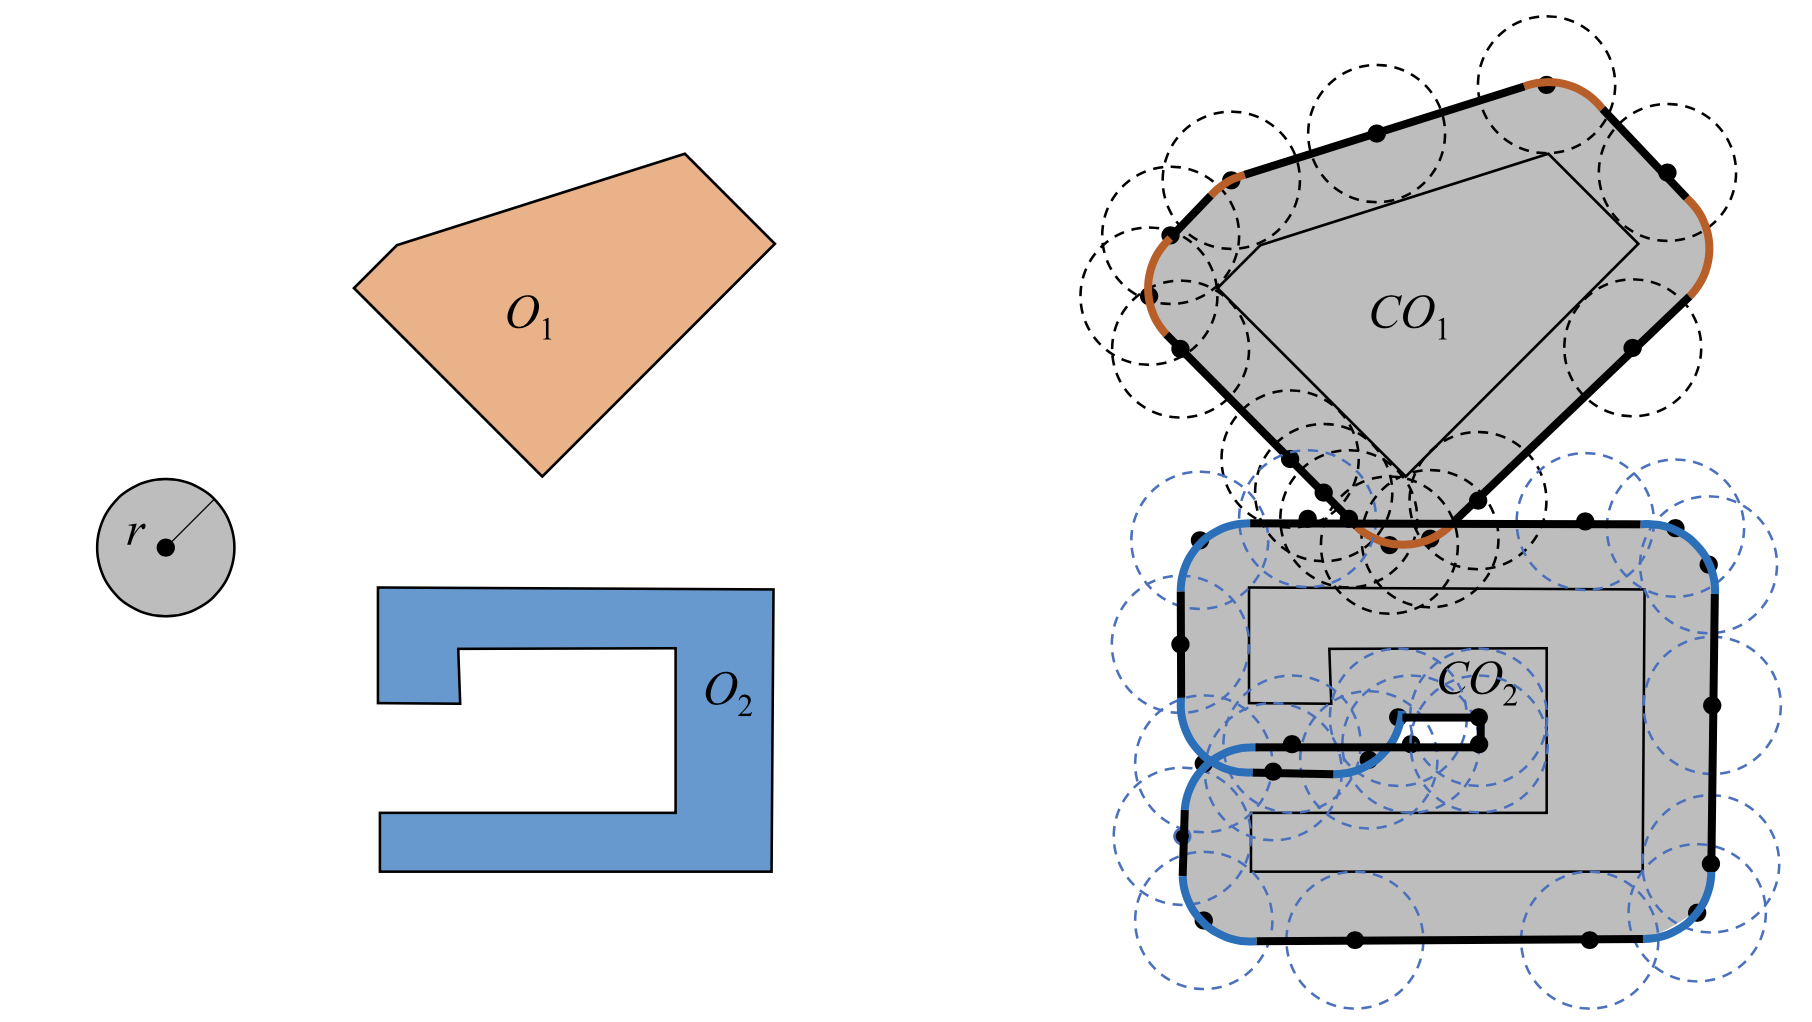
\includegraphics[width= 10 cm]{figures/expanded_obs.png}
        \caption{Consider a disk vehicle with radius $r$ and two obstacles $O_1$ and $O_2$. $CO_1$ and $CO_2$ are the expanded obstacles formed by the Minkowski sum of the vehicle and $O_1$ and $O_2$}
        \label{fig: expand_obs}
    \end{figure*}
    
    
    The algorithm description above is easily applied to point particle vehicles. The situation becomes more involved for 2D non-rotating robots and much more complex if rotational dynamics is accounted for. Instead of applying the point particle formulation of A$^*$ to the center of mass (COM) of the vehicle and performing headache - inducing collision calculations in discrete space, we enlarge the obstacles to account for the vehicle's geometry.  Taking the Minkowski sum of the vehicle and each obstacle produces an enlarged set of obstacles that allows us to apply point particle methods to the vehicle COM, as shown in Figure \ref{fig: expand_obs}. Computing new enlarged obstacles each time the vehicle rotates becomes very mathematically involved; thus, we assume a worst case vehicle - obstacle orientation such that the area of the enlarged obstacle is maximized, leading to a conservative planning algorithm.
    
    The algorithmic workflow proceeds as follows. Once the vehicle and environment geometries are defined, the set of expanded obstacles is computed. The new environment of expanded obstacles is then discretized into a grid of vacant and occupied cells, where occupied cells indicate the presence of an expanded obstacle and unoccupied cells are free for the vehicle to move to. The point vehicle A$^*$ algorithm is then implemented: for each state $x$, all the unoccupied neighboring states (grid points) are found and sorted by their total cost $F(x)$, the vehicle moves to the neighboring state with the lowest $F(x)$, the costs of all states in $Q$ are updated, etc.
    
\section{Software Architecture \& Design Considerations}

\subsection{Runtime Workflow}

Consider the system UML diagram, shown in Figure \ref{fig: UML}. A rough workflow is as follow:

\begin{enumerate}
    \item The user prepares and inputs a config.JSON file, which is parsed by \texttt{Simulator}. \texttt{Simulator} instantiates \texttt{Environment}, \texttt{Agent}, and \texttt{Visualizer}.
    
    \item \texttt{Environment} instantiates the user - specified obstacles from subclasses of \texttt{Obstacle}. \texttt{Agent} instantiates the appropriate vehicle from subclasses of  \texttt{Vehicle} and the specified algorithm from concrete implementations (currently RRT and $A^*$) of the abstract base class \texttt{PathingAlgo}.
    
    \item The chosen planning algorithm attempts to find a feasible or optimal path. \texttt{Agent} checks that the path is consistent with the dynamics and constraints encoded in \texttt{Vehicle}. If a dynamically consistent, feasible path is found, \texttt{Visualizer} animates the result.
    
\end{enumerate}

\subsection{Class Descriptions}

\subsubsection*{Path-Finding Algorithm Class}
The path-finding algorithms are managed via an overarching PathingAlgorithm class which contains each of the different path finding algorithms as subclasses. This was essential to developing modularity within the code, as it allows for each path-finding algorithm to function independent of the different components surround it.


\subsubsection*{Obstacle Class}
The obstacle class is representative of three different shapes available to the user. These three shapes include: a rectangle, circle, and triangle. These obstacles are generated via an Obstacle Factory which takes in the obstacle data from the configuration file and simulator, and generates the appropriate class based on the input data. Note that each of the obstacle classes contains a render method which returns a shape and is used by the Visualizer class. The obstacle classes are as follow:\\

\noindent \textbf{rectangleObstacle}: A rectangular obstacle is represented by an origin point (the bottom left corner of the rectangle), a length, and a width value. This class contains the following attributes:
\begin{itemize}
    \item{shape - this shape attribute is used to distinguish between classes internally}
    \item{length - the length x of the rectangle}
    \item{width - the length y of the rectangle}
\end{itemize}

\noindent \textbf{circleObstacle}: A circular obstacle is represented by a single pair of coordinates which represents the center of the circle and a value that represents its radius. This class contains the following attributes:
\begin{itemize}
    \item{shape - this shape attribute is used to distinguish between classes internally}
    \item{radius - the radius of the circle}
\end{itemize}

\noindent \textbf{triangleObstacle}: A triangular obstacle is represented by three coordinate pairs, each representing one of its vertices. This class does not have any attributes other than its vertices. \\

\begin{figure*}[!h]
    \centering
    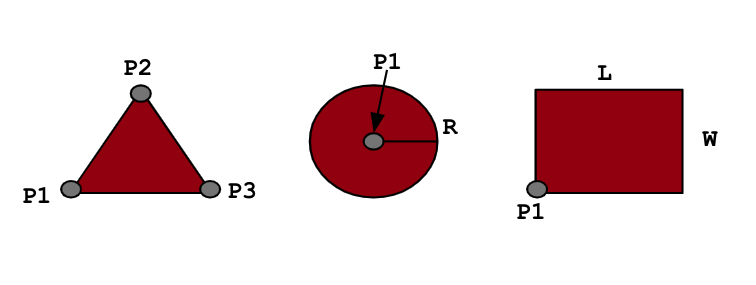
\includegraphics[width= 11 cm]{figures/obstacles.png}
    \caption{Obstacle Class}
    \label{fig: obstacle}
\end{figure*}



\subsubsection*{Vehicle Class}
The vehicle class describes the physical capabilities and size of each vehicle. These are crucial for checking the constraints of each move determined by the path-planning algorithm. Each of the vehicles within the vehicle class also contain a render function which allows them to be drawn and animated at different time-steps via the Visualizer class. \\

\noindent \textbf{Car}: The car was modeled using a Dubins dynamics model. This model defines the dynamic constraints for a car which can only travel forward. This was used a simplified model of a car, with $u$ as the $\theta$ as the orientation angle (relative to the x axis), forward velocity, and $\phi$ as the turn angle. Additionally, $x$ and $y$ determine the position of the center of the rectangular vehicle. For the purposes of simplifying the problem, the velocity input was set to be constant at a value of 1. In order to simulate dynamics that would be considered realistic for a car, the turn angle input was bounded between (and excluding) $-\frac{\pi}{2}$ and $\frac{\pi}{2}$. The dynamics are then given by the following system: 

\begin{itemize}
    \item {$\dot x = u \cos(\theta)$}
    \item {$\dot y = u \sin(\theta)$}
    \item {$\dot \theta = \frac{u}{L} \tan(\phi)$}
\end{itemize}

\noindent \textbf{Unmanned Aerial Vehicle (UAV)}: The UAV or drone is represented by simple dynamics that give it complete dynamic freedom in the $X-Y$ plane. This is largely due to the differential flatness of the UAV dynamics that allow it to travel bounded only by its control inputs. The dynamics of the UAV are given by the following:

\begin{itemize}
    \item{$\dot x = u$}
    \item{$\dot y = v$}
\end{itemize}


\subsubsection*{Agent Class}
This class operates by computing a path to the goal and comparing the path with the possible dynamics of the chosen vehicle. Due to the inheritance structure, the agent is agnostic to both the algorithm used and the dynamics of the chosen vehicle. It calculates a trajectory by, at every timestep, recalculating the path to the goal set and comparing the dynamics for a single move along that path. This process is continued until the vehicle is in the goal set or a simulation timing requirement has been met. In this way, a dynamically-valid trajectory is generated.



\subsubsection*{Environment Class}
\noindent The environment class contains the dimensions of the domain as well as a list of obstacles that exist within the bounds of the environment. 

\begin{figure*}[!h]
    \centering
    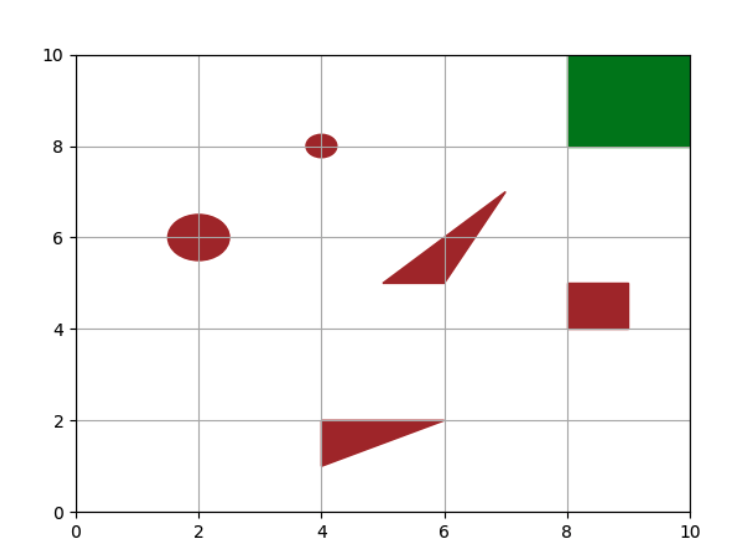
\includegraphics[width= 7 cm]{figures/env1.png}
    \caption{Environment Render}
    \label{fig: env1}
\end{figure*}


\subsubsection*{Simulator Class}
This class constitutes the driver of the trajectory planning code. It takes in a JSON configuration file location and parses it into multiple dictionaries that are distributed to the agent and the environment. It makes use of a simple API composed of 2 functions: run() and animate(). Run attempts to validate whether or not a trajectory from the initial position to the goal position is possible in the given time constraint and animate creates a visual representation of the trajectory.


\subsection*{Static Environment}
We classify obstacles into two main categories: static and dynamic obstacles. Static obstacles' position does not depend on time, as they are stationary based on their initial position.

\subsection*{Dynamic Environment}
The second category of obstacles are considered dynamic obstacles where their position is dependent on time. These kinds of obstacles would be passed into the configuration file with accompanying functions that determine this position over time. While these kinds of obstacles were not implemented into the current iteration of the program, this serves as an important foundation for future work. 



\section{Development Process}
\subsection{Initial Project Planning}
The initial idea went through many project iterations before it was decided upon. It took a while and several meetings to specifically nail down just what this project should be. Once that had been decided, a coalition was formed to decide the overall design structure and high level UML diagram of the code. This UML was refined and reworked in later meetings. In general, the approach taken with regards to planning was a very fluid one. This can undermine a team easily, but thanks to strong communication and constant self-accountability, we were able to manage the workflow well and hit project goals. 

\subsection{Choosing a Language}
Python was chosen for this project due to its ubiquity and ease of use. Specifically, it was felt that python balanced power with ``friendliness". This so-called ``friendliness" was a big concern for some of our group as there were several members who had very little programming experience prior to this class. At the same time, there were several members who were relatively experienced in python which made it ideal for teaching. Besides this fact, the ability to rapidly develop coding solutions is more tuned to python than other languages such as C due to its low barrier to entry.

\subsection{Setting up Git}
We chose to use Github actions for our continuous integration platform. The flexibility of on-commit testing allowed for the opportunity of better working code to be produced. Despite this, our inexperience in AGILE practices, and particularly in code development and testing hampered our ability to utilize it to the fullest. More primitive git tools proved more effective, however. Git branching was used effectively to partition and modularize the code through out the development process. We specifically used a workflow that relied on multiple module development branches that were merged into one super development branch before being pushed to main. This solution was chosen because it was seen as a more streamlined solution than a more complex branching practice involving pull requests. The benefit to this is it kept any sort of git mishaps relatively shielded from the rest of the code base which helped to minimize our merge errors.

\subsection{Applying Documentation Through Sphinx}
This was also an introductory experience to learning proper documentation practices and learning how to use Sphinx to produce finished documentation products. We used Sphinx as it is most suited for documenting Python code. Sphinx-quickstart \texttt{--auto-doc} was used to provide the initial scaffolding of configuration and build files, providing us with the basic Makefile, conf.py, and index.rst function. Sphinx-apidoc was then used to generate .rst files based on the modules present.\\

\noindent The conf.py file is highly customizable and critical for generating outputs. All basic project information in included in this file, such as the project title, copyrights, author names, and versions. In this file, we also enabled a variety of extensions to accommodate our project needs. For example, we included the Napoleon extensions, which enables Sphinx to parse both NumPy and Google style docstrings. We also included Intersphinx linking, which generates automatic links to the documentation of objects in other projects, or help crosslink different libraries. The conf.py file also allows us to adjust how the HTML or LaTeX PDF files will output and what the formatting constraints look like. This file can be readily adjusted and more functions can be added if the project is expanded or there is a need other types of output files.\\

\noindent The index.rst file provides the front page of the HTML output and also structures the toctree, or a "Table of Contents tree", that provides the layout for the rest of the .rst files. This is where the modules are organized. Here, we are also able to link together other parts of the project, such as the Git repository or Overleaf Final Report. Overall, this enables a better organization of the Sphinx documentation and allows the users to better understand the software package.\\ 

\noindent As noted in the Sphinx documentation and README, users can generate either an HTML output or LaTeX PDF file for the documentation of the code. Directions for doing so are located in the README and again reiterated in the Sphinx documentation. 

\section{Lessons Learned}
Throughout the process there were many valuable lessons and experiences that helped with optimizing our processes. 

\subsection*{Adjusting to Different Skill Levels and Backgrounds}
Our team has members with a variety of different backgrounds and experience with coding, so there were some difficulties adjusting the project so that all members were able to understand and participate. For example, one of our team members had very little experience in coding and did not have a STEM background, so we needed to adjust the project so that everyone was able to work together and generate the software package. This was one of the hiccups we faced when trying to decide on the initial project idea, since there were many ideas but not many that all members were good with. Adjustments were made, but looking forward, the workflow would have been smoother if everyone had been brought up to speed a lot earlier in the process (or a lot earlier in the semester, in this situation, as opposed to the schedule that was planned out in the syllabus). However, it was still a great learning experience interfacing with all the different aspects involved in developing a piece of software collaboratively. 

\subsection*{Understanding and Managing Git Workflow}
Although we have had prior experience using Git repositories and understanding the basic mechanics of pulling and pushing content, this was the first time we had to maintain our own repository and coordinate collaboration with multiple team members simultaneously. The initial set-up of the repository was managed by one individual, where we experienced some challenges in trying to set up the repository to package the project and automate testing. There were more configuration files needed than initially expected, but we were otherwise able set up the foundation for the repository.\\

\noindent Moving forward, we decided for each class or subclass that was being worked on, we would create a branch and separate the workflow based on who was assigned what part of the project. The general objective was to ensure clean division of the tasks and maintaining the integrity of the code. There was a slight learning curve in the beginning as we branched out and started working on different sections. There were some initial branching issues and confusion over what branch was where, and some issues ending up with branches that were unnecessary or cluttering up the repository. However, those issues were generally resolved and enabled cleaner and consistent workflow to minimal collisions between the different branches. 




\section{Future Work}
The majority of future work for this project will involve expanding the flexibility and freedom that the user has in choosing their inputs. This concept can be applied specifically to the vehicle, pathing algorithm, and obstacle classes. Currently, the program provides path planning using the UAV whose dynamics allow for movement only limited by its control input. However, for more complex applications such as autonomous driving, the implementation of dynamic constraints into the vehicle are vital to understanding the physical limitations of the vehicle as it moves through the pre-planned path. This can be done in a similar fashion for the pathing algorithm class via the implementation of other more complex and efficient algorithms such as Random Walk and D*. This would further provide the user with the ability to choose the optimal or standard algorithm used for their specific industry or application. \\

\noindent In the context of the obstacle class, further work can be done to improve the flexibility in choosing the shapes of said obstacles as well as the addition of dynamic obstacles. The idea behind dynamic environments is that each obstacle has an accompanying time-dependent function that allows the agent to track its movement at each time step. This increases the complexity of the code significantly, especially if we allow the agent to determine different control inputs for the vehicle. However, this complex case is perhaps more relevant in real-world applications where, for example, a car must find an optimal path in while other vehicles are moving around it. Beyond improvement of the actual capabilities of each class within the program, future work could involve the introduction of machine and deep learning for determining the optimal path algorithm given the vehicle and environment conditions provided. This could be implemented via a neural network that is trained on data representing path-planning problems and the optimal or standard path planning algorithm for the given environment. This can be vital to providing a tool that can not only path plan, but do so using optimal conditions. 



\printbibliography 
\nocite{*}
\end{document}
